\documentclass{article}

\usepackage[%
    left=0.5in,%
    right=0.5in,%
    top=0.5in,%
    bottom=0.5in,%
]{geometry}%
\usepackage{minitoc}
\usepackage{multicol}
\usepackage{graphicx}
\usepackage{fixltx2e}
\usepackage{listings}
\usepackage{color}
\usepackage{hyperref}
    \hypersetup{ colorlinks = true, linkcolor = blue }
\usepackage{blindtext}
\definecolor{lightgray}{gray}{0.9}
\graphicspath{ {./} }

\newcommand{\inlinecode}[2]{\colorbox{lightgray}{\lstinline
[language=#1]$#2$}}
\newcommand{\worddef}[1]{\hyperref[sec:reference]{\textit{#1}}}

\begin{document}

\tableofcontents

\newpage

\section{Firewalls}
\begin{itemize}
  \item A hardware and/or software system 
  \item Prevents unauthorised access of packets from one network to another 
  \item \textbf{All data leaving any subnet must pass through it}
\end{itemize}

\subsection{Firewall Functions}
\begin{itemize}
  \item Implements ‘single point’ security measures 
  \item Security event monitoring through packet analysis and logging 
  \item Network-based access control through implementation of a rule set
\end{itemize}

\section{Location}  
\begin{itemize}
  \item Network Firewalls: Placed between a subnet and the internet  
  \item Host-based Firewalls: Placed on individual machines
  \item A standard home router is a good example of a \textit{network firewall}
  \item A \textit{demilitarized zone} is a small subnet that\textbf{ separates externally facing
services} from the internal network
\end{itemize}

\section{Firewall Basic Function}
\begin{itemize}
  \item Defends a network against parties accessing internal services 
  \item Can also restrict access from \textbf{inside to outside services} (e.g. IRC, P2P) 
  \item Network Address Translation: \textbf{hides the internal machines} with private addresses
\end{itemize}

\subsection{Firewalls are not enough}
\begin{itemize}
  \item Cannot protect against attacks that \textbf{bypass the firewall}. E.g. Tunnelling 
  \item Cannot protect against \textbf{internal threats} or insiders. Might help a bit by egress filtering 
  \item Network firewalls cannot always \textbf{protect against the transfer} of virus-infected programs or files
\end{itemize}

\section{Packet Filters}
\begin{itemize}
  \item Specify which packets are allowed or dropped 
  \item Rules based on: source / destination IP, TCP / UDP port numbers 
  \item Possible for both inbound and outbound traffic 
  \item Can be implemented \textbf{in a router} by only examining packet headers (IP / TCP)
\end{itemize}

\subsection{Packet Filter Rules}
\begin{itemize}
  \item Rule execution depends on implementation 
  \begin{itemize}
    \item IPTABLES: First rule to match is applied 
    \item PF: All rules are examined, the last match is applied 
  \end{itemize}
  \item Rules are organised in chains, which are logical subgroups of rules 
  \item Depending on the packet, different chains are activated
\end{itemize}

\subsection{IPTABLES}
\begin{itemize}
  \item An application that provides access to the Linux firewall rule tables 
  \item \textbf{Not actually a firewall}, but configures the firewall 
  \item The firewall is mostly implemented as \textit{netfilter} modules
\end{itemize}

\subsection{Tables and Chains}
\begin{multicols}{2}
\begin{itemize}
  \item IPTABLES uses tables to store chains.Default is the filtering table 
  \item Chains are ordered lists of rules. Rules match, or they don’t 
  \item Matches result in a \textbf{jump}, else we check the next rule
  \item There can be multiple chains per table. E.g. a TCP handling chain 
  \item Jumps can go to ACCEPT, DROP, LOG or another chain 
  \item Complex behaviour can be built up
\end{itemize}
\begin{center}
  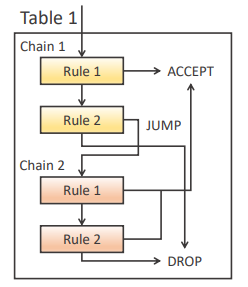
\includegraphics[scale=0.7]{table_chain.png}
\end{center}
\end{multicols}

\subsection{Defaults}
\begin{itemize}
  \item There are four built-in tables in IPTABLES: \textbf{Filter, NAT, Mangle – Packet alteration, Raw – Skips connection tracking}
  \item The default table is the \textbf{filtering table}, including Input, Output and Forward chains
\end{itemize}

\subsection{Example}
\begin{itemize}
  \item Using the command line, we add rules onto the end of chains
  \item \verb!iptables -A INPUT -i eth0 -p tcp --dport 80 -j ACCEPT!
  \item \verb!iptables -A OUTPUT -o eth0 -p tcp --sport 80 -j ACCEPT!
\end{itemize}

\pagebreak

\subsection{Policies}
\begin{itemize}
  \item Permissive (Black listing) – allow everything \textbf{except dangerous services}. Easy to make a mistake or forget something 
  \item Restrictive (White listing) – block everything except designated useful services 
  \begin{itemize}
    \item More secure by default 
    \item Fairly easy to DoS yourself!
  \end{itemize}
  \item To use a blacklisting policy, we want to accept by default, then have rules that drop:
  \begin{itemize}
    \item iptables -P INPUT ACCEPT
    \item iptables -P FORWARD ACCEPT
    \item iptables -P OUTPUT ACCEPT
    \item iptables -A INPUT -s X.X.X.X” -j DROP
    \item iptables -A OUTPUT -p tcp --dport ssh -j DROP
  \end{itemize}
  \item For a whitelisting policy, we want to drop by default, then let certain packets through:
  \begin{itemize}
    \item iptables -P INPUT DROP
    \item iptables -P FORWARD DROP
    \item iptables -P OUTPUT DROP
    \item iptables -A INPUT -p tcp --dport ssh -j ACCEPT
    \item iptables -A OUTPUT -s 192.168.0.2” -j ACCEPT
  \end{itemize}
\end{itemize}

\section{Packet Filter Issues}
\begin{itemize}
  \item Packet filters are simple, low level and have high assurance 
  \item \textbf{But, they cannot:}
\begin{itemize}
  \item Prevent attacks that employ \textbf{application-specific vulnerabilities} 
  \item Do not support higher-level \textbf{authentication schemes} 
  \item Easy to \textbf{accidentally allow or deny} packets incorrectly
\end{itemize}
\end{itemize}

\subsection{Stateful Packet Filters}
\begin{itemize}
  \item Understand requests and replies (e.g. ACK/SYN) 
  \item \textbf{Dynamically generate rules} 
  \item E.g. FTP client, connect to 21, receive from 20 
  \item Can support policies for a wider range or protocols
\end{itemize}

\subsection{IPTABLES Rules}
\begin{itemize}
  \item IPTABLES has modules for stateful packet filtering 
  \item Allow incoming / outgoing SSH connections
  \begin{itemize}
    \item iptables -A INPUT -i eth0 -p tcp --dport 22 -m state --state NEW,ESTABLISHED -j ACCEPT
    \item iptables -A OUTPUT -o eth0 -p tcp --sport 22 -m state --state ESTABLISHED –j ACCEPT
  \end{itemize}
  \item Allow HTTP(S):
  \begin{itemize}
    \item iptables -A INPUT -i eth0 -p tcp --dport 80 -m state --state NEW,ESTABLISHED -j ACCEPT
    \item iptables -A OUTPUT -o eth0 -p tcp --sport 80 -m state --state ESTABLISHED -j ACCEPT
    \item iptables -A INPUT -i eth0 -p tcp --dport 443 -m state --state NEW,ESTABLISHED -j ACCEPT
    \item iptables -A OUTPUT -o eth0 -p tcp --sport 443 -m state --state ESTABLISHED -j ACCEPT
  \end{itemize}
  \item ACK packets are used to keep \textbf{track of the session} – the connection is ongoing 
  \item Packets without the ACK are the \textbf{connection establishment messages}
\end{itemize}

\section{Application-level Gateways}
\begin{itemize}
  \item Packer filters have limited criteria that allow data in and out 
  \item An application gateway considers the \textbf{application-layer} protocol that is in use 
  \item Some protocols, like HTTP and SSH will be allowed, others, like BitTorrent, may be blocked 
  \item Can perform much \textbf{more complex port control} than fixed rules
\end{itemize}

\section{Proxy Servers}
\begin{itemize}
  \item Proxy servers initiate a connection on our behalf 
  \item They can block certain access, and scan for malicious files or web pages
  \item Issues:
  \begin{itemize}
    \item Large overhead per connection 
    \item More expensive than packet filtering 
    \item Configuration is complex 
    \item A separate server is required for each service
  \end{itemize}
\end{itemize}

\section{Network Address Translation}
\begin{itemize}
  \item The shortage of IP addresses mean that most routers now perform NAT automatically
  \item Meaning: only the router has an ip \textbf{visible to the world}, all machines within the network get assigned an ip by the router.
  \item The implicit advantage in NAT is that your machine is almost totally hidden from the internet 
  \item Only established connections are forwarded to your internal machine 
  \item Or, specific port forwarding rules 
  \item This\textbf{ prevents any unsolicited attacks} on random ports, but no other types of attack
\end{itemize}

\section{Host-Based Firewalls}
\begin{itemize}
  \item The router firewall could break at any time, leaving all other machines to be vunerable
  \item If a machine get's a virus, then router firewall can't stop other in-network machines from getting affected.
  \item When plugging in to a public network, there is no protection from router and the network itself might be malicious
\end{itemize}

\pagebreak
\section*{Reference section} \label{sec:reference}
\begin{description}
	\item[placeholder] \hfill \\
\end{description}
\end{document}
